\documentclass[12pt]{article}

\newcommand{\danger}{\tikz[baseline=-.75ex] \node[color=red, shape=regular polygon, regular polygon sides=3, inner sep=0pt, draw, thick] {\textbf{!}};}

\input{etc/cmd}

\begin{document}
\fontsize{12pt}{14pt}\selectfont

\input{etc/head}

هدف از این آزمایش آشنایی با گیت‌های منطقی و تحلیل مدار‌های ساده ترکیبی است.

\section{قطعات و تجهیزات}
\begin{itemize}
    \item آی‌سی \lr{7404} 
    \item آی‌سی \lr{7408} 
    \item آی‌سی \lr{7432}
    \item ماژول \lr{Dig Inverter}
    \item مقاومت‌های ۲۲۰ اهمی 
    \item \lr{LED}
    \item بردبورد
    \item سیم جامپر
    \item منبع تغذیه
    \item مولتی‌متر
    \item سیگنال ژنراتور
    \item اسیلوسکوپ
\end{itemize}

\section{پیش مطالعه}
در این آزمایش با گیت‌های منطقی پایه و تجهیزات آزمایشگاه آشنا خواهید شد. پیشنهاد می‌شود پیش از انجام آزمایش‌ها، دیتاشیت مربوط به هر آی‌سی را مطالعه کنید تا آزمایش‌ها را سریع‌تر و با دقت بیشتری انجام دهید. چند نکته:

\begin{itemize}
    \item  در آزمایشگاه این درس هر کجا ولتاژ منطقی \lr{"0"} و \lr{"1"} ذکر شد، به ترتیب منظور ولتاژ زمین مدار 
و ولتاژ 5 ولت می باشد.
    \item در درس مدارهاس الکتریکی با بردبورد و نحوه اتصالات آن آشنا شدید. از آنجایی که سوراخ‌های آن به طور عمودی به همدیگر متصل شده‌اند، به سادگی می‌توان قطعات الکترونیکی را بر روی آن قرار داد و برای برقراری اتصالات از هر ستون به ستون دیگر، از سیم‌های جامپر کمک گرفت. 
    \item در اتصالات مدار‌های خود بر روی بردبورد، سعی کنید تا جای ممکن جامپرهای کمتری استفاده 
کنید.
    \item برد مدار چاپی \lr{(Printed Circuit Board)} صفحه‌ای از جنس معمولا فایبرگلاس است که اتصالات بین قطعات بر روی آن حک شده، قطعات الکترونیکی مانند مقاومت، خازن و سلف بر روی آن مونتاژ شده و جهت استفاده در تجهیزات الکتریکی به کار گرفته می‌شود. در بخشی از این آزمایش، نمونه‌ای از یک برد \lr{PCB} در اختیار شما قرار خواهد گرفت تا آزمایش را ساده‌تر انجام دهید.
    \item برای شناسایی پایه‌های \lr{LED} از شکل زیر کمک 
بگیرید. 

    \item[\danger] به منظور جلوگیری از سوختن \lr{LED}های قرمز استفاده از مقاومت‌های محدودکننده ۲۲۰ اهمی را هرگز  فراموش نکنید!
\end{itemize}
\begin{figure}[!h]
    \centering
    \includegraphics[width=0.5\linewidth]{figs/led.jpg}
\end{figure}

\section{دستور کار}
\subsection{آشنایی با تجهیزات آزمایشگاه مدارهای منطقی (۲۰ دقیقه)}
\begin{itemize}\item
هدف از انجام این بخش از ‌آزمایش، آشنایی با اسیلوسکوپ‌های آنالوگ و دیجیتال، سیگنال ژنراتور و مولتی‌متر است که ابزار اولیه مورد استفاده در آزمایش‌های درس مدار‌های منطقی بوده و تسلط بر آن‌ها مهم است.
\item تحویل این بخش از آزمایش اجباری نیست. پیشنهاد می‌شود که به منظور مرور مطالب درس مدار‌های الکتریکی، آن را انجام دهید. درصورتی که به این تجهیزات تسلط کامل دارید، می‌توانید به سراغ بخش بعدی آزمایش بروید.
\end{itemize}

\subsubsection{آشنایی با مولتی‌متر}
\begin{itemize}
    \item مولتی‌متر دستگاهیی برای اندازه‌گیری پارامتر‌های مدار‌های الکتریکی اعم از ولتاژ، جریان و مقاومت است که معمولا امکانی برای تست اتصالات مدار، اندازه‌گیری ظرفیت خازن و ... را نیز شامل می‌شود.
    \item ابتدا مولتی‌متر را بر روی اهم تنظیم کنید و مقاومت چند عدد مقاومت کربنی با مقاومت نامی ۲۲۰ اهم و ۱۰۰ اهم را اندازه‌گیری کنید. مقادیر اندازه‌گیری شده را با مقادیر نامی مقایسه کنید و درصد خطا را بدست آورید. آیا این درصد خطا در محدوده خطای ذکر شده روی مقاومت است؟ آیا مقاومت‌های آبی‌رنگ، با مقاومت‌های کرم‌رنگ متفاوت‌اند؟
    \item مدار شکل ۱ را به وسیله دو مقاومت روی برد آزمایشگاه ببندید. مولتی‌متر را روی اندازه‌گیری ولتاژ تنظیم کرده و ولتاژ نقاط \lr{A}، \lr{B}، و \lr{C} را اندازه‌گیری کنید و با مقادیر محاسبه‌شده آن‌ها مقایسه نمایید. خطای اندازه‌گیری را بدست آورید. این خطا از چه چیزی ناشی شده است؟
    \begin{figure}[!h]
        \centering
        \includegraphics[width=0.5\linewidth]{figs/circuit.png}
        \caption{مدار تقسیم ولتاژ با مقاومت}
        \label{fig:1}
    \end{figure}
\end{itemize}

\subsubsection{آشنایی با اسیلوسکوپ و سیگنال ژنراتور}
\begin{itemize}
    \item در درس آزمایشگاه مدار‌های الکتریکی، نحوه با کار اسیلوسکوپ و سیگنال ژنراتور را که به ترتیب جهت نمایش و تولید سیگنال‌ها استفاده می‌شوند را آموختید. به منظور یادآوری مجدد قابلیت‌های آن‌ها می‌توانید به \href{www.google.com}{این سند} مراجعه کنید.
    \item موج کالیبراسیون اسیلوسکوپ را روی نمایشگر آن نمایش دهید. سیگنال ورودی را روی حالت‌های \lr{AC Coupled} و \lr{DC Coupled} قرار دهید و تفاوت ایجاد شده را توجیه کنید. به نظر شما هر یک از این گزینه‌ها چه کاربردی دارند؟
    \item با استفاده از سیگنال ژنراتور، موج مربعی با فرکانسی در حدود ۱۰-۱۰۰ کیلوهرتز تولید کنید و روی اسیلوسکوپ نمایش دهید. دامنه و فرکانس موج تولیدی را با کمک خانه‌های صفحه نمایش‌گر اسیلوسکوپ بدست آورید.
\end{itemize}

\subsection{کار با آی‌سی \lr{7404} (۳۰ دقیقه)}
\begin{itemize}
    \item آی‌سی \lr{7404} را در جای مناسبی از بردبورد قرار دهید.
    \item پین‌های تغذیه آی‌سی را شناسایی کرده و به آن ولتاژ ۵ ولت دی‌سی اعمال کنید (به شکل ۱ مراجعه کنید.)
    \begin{figure}[!h]
        \centering
        \includegraphics[width=0.5\linewidth]{figs/7404.png}
        \caption{پین‌های آی‌سی}
        \label{fig:1}
    \end{figure}
    \item در این آی‌سی ۶ گیت منطقی وجود دارد. ورودی یکی از این گیت‌ها پین ۱ و خروجی آن پین ۲ می‌باشد.
    \item به ورودی این آی‌سی یک‌ بار ولتاژ منطقی \lr{"0"} و بار دیگر ولتاژ منطقی \lr{"1"} را اعمال کنید. تغییرات خروجی را نسبت به ورودی‌های اعمالی یادداشت کنید. برای راحتی کار پیشنهاد می‌شود در ورودی و خروجی این آی‌سی یک \lr{LED} به همراه یک مقاومت ۲۲۰ اهم به صورت سری متصل کنید. نمونه‌ای از این مدار را در شکل ۲ مشاهده می‌کنید (با استفاده از حالت اهم‌متر مولتی‌متر، از ۲۲۰ اهم بودن مقاومت اطمینان حاصل کنید).
    
    \begin{figure}[!h]
        \centering
        \includegraphics[width=0.5\linewidth]{figs/not.png}
        \caption{مدار نمونه بخش اول}
        \label{fig:2}
    \end{figure}
    
    \item مولتی‌متر را روی حالت ولت‌متر تنظیم کرده و پس از اعمال ورودی‌های \lr{"0"} و \lr{"1"} منطقی، در هر حالت ولتاژ خروجی را اندازه‌گیری کرده و یادداشت کنید.
\end{itemize}

\subsubsection{کار با ماژول \lr{Dig Inverter}}
در طراحی مدارات دیجیتال و آنالوگ، بهینه‌سازی مساحت مصرفی و طول اتصالات از اهمیت بالایی برخوردار است. در صنعت الکترونیک، بعد از صحت‌سنجی عملکرد مدار بر روی بردبورد و اطمینان از آن، به مرحله طراحی و ساخت برد مدار چاپی (\lr{Printed Circuit Board}) می‌رسیم.

در شکل ۴، تصویری از ماژول \lr{Dig Inverter} که در اختیار دارید را می‌بینید. این برد به منظور کار ساده‌تر با آی‌سی \lr{7404} و همچنین محافظت از آن در برابر تغذیه معکوس و یا بیشتر از میزان ولتاژ نامی طراحی شده‌است. 
\begin{figure}[!h]
    \centering
    \includegraphics[width=0.7\linewidth]{figs/pcb.jpg}
    \caption{ماژول \lr{Dig Inverter}}
    \label{fig:3}
\end{figure}
\begin{itemize}
    \item پین \lr{VCC} آی‌سی را به خروجی منبع تغذیه و پین \lr{Gnd} را به زمین آن متصل کنید و خروجی منبع تغذیه را بر روی ۹ ولت \lr{DC} تنظیم کنید.  
    \item این‌بار یکی از گیت‌ها را از بردی که اختیار دارید انتخاب کرده و مقادیر منطقی \lr{"0"} و \lr{"1"} به ورودی آن اعمال کنید.
    \item مقادیر خروجی آی‌سی \lr{7404} را در بخش قبل با مقادیر بدست‌آمده از این برد مقایسه کنید و از صحت عملکرد آ‌ی‌سی اطمینان حاصل کنید.
\end{itemize}

\subsubsection{بدست‌ ‌آوردن مشخصه خروجی گیت \lr{NOT}}
مشابه بخش قبلی، پایه وسط یک پتانسیومتر ۵ کیلو‌اهم را به ورودی گیت متصل کنید و دو اتصال دیگر را به زمین و ولتاژ ۵ ولت \lr{DC} وصل کنید. با تغییر پتانسیومتر، ولتاژ اعمالی به ورودی گیت از ۰ تا ۵ ولت تغییر می‌کند. در حین تغییر پتانسیو‌متر، ولتاژ خروجی گیت را اندازه‌گیری کنید؛ در منطقه‌ای که تغییر ولتاژ سریع است، تعداد نقطه‌های بیشتری را اندازه‌گیری کنید. سپس مشخصه خروجی بر حسب ورودی را برای گیت رسم کنید. با توجه به مشخصه، محدوده‌های ولتاژ مربوط به ناحیه ولتاژ منطقی \lr{"0"} و \lr{"1"} را تعیین کرده و آن‌ها را با مقادیر داده‌شده در دیتاشیت مقایسه کنید.

\subsection{بررسی جدول صحت آی‌سی \lr{7408} (۱۵ دقیقه)}
\begin{itemize}
    \item آی‌سی \lr{7408} یک گیت \lr{AND} چهارگانه است به گونه‌ای که ۴ جفت ورودی و ۴ خروجی دارد. حال این آی‌سی را در جای مناسبی از بردبورد قرار دهید.
    \item پین‌های تغذیه آی‌سی را شناسایی کرده و به آن ولتاژ ۵ ولت \lr{DC} اعمال کنید.
    \item پین‌های مربوط به یکی از گیت‌های این آی‌سی را شناسایی کنید و سپس در هریک از ورودی‌ و خروجی‌های آن، یک \lr{LED} به همراه یک مقاومت ۲۲۰ اهم سری قرار دهید.
    \item به ورودی‌های این گیت به ازای تمام حالات (جدول ۱)، ولتاژ منطقی \lr{"0"} و \lr{"1"} اعمال کنید و برای هر حالت، خروجی گیت را یادداشت کنید.
    \item جدول درستی حاصل از بخش قبل را با عملکرد مورد انتظار مقایسه کنید و از صحت کار آی‌سی اطمینان حاصل کنید.

    \begin{table}[!h]
        \centering
        \renewcommand{\arraystretch}{2}
        \setlength{\tabcolsep}{18pt}
        \LTR
        \begin{tabular}{||c|c|c||} \hline
         \textbf{\lr{Input 1}} & \textbf{\lr{Input 2}} & \textbf{\lr{Output}}\\ \hline
         \lr{0} & \lr{0} & \lr{}\\ \hline
         \lr{0} & \lr{1} & \lr{}\\ \hline
         \lr{1} & \lr{0} & \lr{}\\ \hline
         \lr{1} & \lr{1} & \lr{}\\ \hline
        \end{tabular}
        \RTL
        \caption{جدول درستی آی‌سی \lr{7408}}
        \label{tab:1}
    \end{table}
\end{itemize}

\subsection{بررسی صحت خروجی مدار ترکیبی (۳۰ دقیقه)}
\begin{itemize}
    \item در بخش‌های قبل با ‌آی‌سی‌های \lr{7404} و \lr{7408} که به ترتیب مربوط به گیت‌های منطقی \lr{NOT} و \lr{AND} بودند آشنا شدیم. در این بخش، به کمک این دو آی‌سی و همچنین گیت منطقی \lr{OR} (آی‌سی \lr{7432})، یک مدار ترکیبی خواهیم ساخت.
    \item مدار زیر را ببندید و به ازای تمام ورودی‌های ممکن، خروجی را متناسب با جدول ۲ کامل کنید.
    \begin{figure}[!h]
        \centering
        \includegraphics[width=0.5\linewidth]{figs/comb.png}
        \caption{مدار ترکیبی}
        \label{fig:3}
    \end{figure}
    
    \begin{table}[!h]
        \centering
        \renewcommand{\arraystretch}{2}
        \setlength{\tabcolsep}{18pt}
        \LTR
        \begin{tabular}{||c|c|c|c|c||} \hline
         \textbf{\lr{a}} & \textbf{\lr{b}} & \textbf{\lr{c}} & \textbf{\lr{f(0/1)}} & \textbf{\lr{f(volt)}} \\ \hline
         \lr{0} & \lr{0} & \lr{0} & \lr{} & \lr{}\\ \hline
         \lr{0} & \lr{0} & \lr{1} & \lr{} & \lr{}\\ \hline
         \lr{0} & \lr{1} & \lr{0} & \lr{} & \lr{}\\ \hline
         \lr{0} & \lr{1} & \lr{1} & \lr{} & \lr{}\\ \hline
         \lr{1} & \lr{0} & \lr{0} & \lr{} & \lr{}\\ \hline
         \lr{1} & \lr{0} & \lr{1} & \lr{} & \lr{}\\ \hline
         \lr{1} & \lr{1} & \lr{0} & \lr{} & \lr{}\\ \hline
         \lr{1} & \lr{1} & \lr{1} & \lr{} & \lr{}\\ \hline
        \end{tabular}
        \RTL
        \caption{جدول درستی مدار ترکیبی}
        \label{tab:2}
    \end{table}
\end{itemize}

\subsection{تجزیه و تحلیل عملکرد مدار ترکیبی (۲۰ دقیقه)}
\begin{itemize}
    \item آی‌سی \lr{7486} مربوط به گیت منطقی \lr{XOR} می‌باشد. 
    \item مدار شکل ۶ را بر روی بردبورد ببندید.
    \item همان‌طور که مشاهده‌ می‌کنید، این مدار ۲ عدد خروجی دارد. خروجی‌های آن را به ازای مقادیر مختلف ورودی‌های آن بررسی کنید. به نظر شما، این مدار چه کاربردی دارد؟
\end{itemize}




\tikzset{every picture/.style={line width=0.75pt}} %set default line width to 0.75pt   
\begin{center}
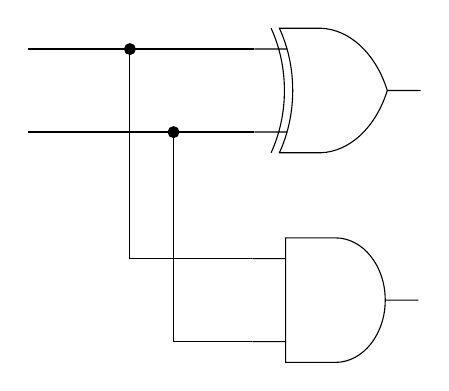
\begin{tikzpicture}[x=0.75pt,y=0.75pt,yscale=-1,xscale=1]
%uncomment if require: \path (0,211); %set diagram left start at 0, and has height of 211
%Shape: Xor Gate [id:dp9102031764758916] 
\draw   (357,24) -- (377,24) .. controls (390.95,24.54) and (403.42,36.23) .. (409,54) .. controls (403.42,71.77) and (390.95,83.46) .. (377,84) -- (357,84) .. controls (365.57,65.44) and (365.57,42.56) .. (357,24) -- cycle (345,34) -- (361,34) (345,74) -- (361,74) (409,54) -- (425,54) (353,24) .. controls (361.57,42.56) and (361.57,65.44) .. (353,84) ;
%Shape: And Gate [id:dp766696587274974] 
\draw   (360,125) -- (384,125) .. controls (397.25,125) and (408,138.44) .. (408,155) .. controls (408,171.56) and (397.25,185) .. (384,185) -- (360,185) -- (360,125) -- cycle (344,135) -- (360,135) (344,175) -- (360,175) (408,155) -- (424,155) ;
%Straight Lines [id:da8292378154834694] 
\draw    (306,175) -- (344,175) ;
%Straight Lines [id:da5551787159328023] 
\draw    (285,135) -- (344,135) ;
%Straight Lines [id:da9712637228882144] 
\draw    (236,74) -- (345,74) ;
%Straight Lines [id:da5267260001623191] 
\draw    (236,34) -- (345,34) ;
%Straight Lines [id:da012125431286500898] 
\draw    (285,135) -- (285,34.05) ;
%Straight Lines [id:da2696971598920219] 
\draw    (306,175) -- (306,74.05) ;
%Shape: Circle [id:dp32930792233284656] 
\draw  [fill={rgb, 255:red, 0; green, 0; blue, 0 }  ,fill opacity=1 ] (282.4,34.05) .. controls (282.4,32.61) and (283.56,31.45) .. (285,31.45) .. controls (286.44,31.45) and (287.6,32.61) .. (287.6,34.05) .. controls (287.6,35.49) and (286.44,36.65) .. (285,36.65) .. controls (283.56,36.65) and (282.4,35.49) .. (282.4,34.05) -- cycle ;
%Shape: Circle [id:dp588573519103307] 
\draw  [fill={rgb, 255:red, 0; green, 0; blue, 0 }  ,fill opacity=1 ] (303.4,74.05) .. controls (303.4,72.61) and (304.56,71.45) .. (306,71.45) .. controls (307.44,71.45) and (308.6,72.61) .. (308.6,74.05) .. controls (308.6,75.49) and (307.44,76.65) .. (306,76.65) .. controls (304.56,76.65) and (303.4,75.49) .. (303.4,74.05) -- cycle ;
\end{tikzpicture}
\end{center}


\subsection{طراحی یک نوسان‌ساز (۲۰ دقیقه)}
\begin{itemize}
    \item توسط دو عدد آی‌سی \lr{7404} و پشت سر هم بستن ۱۱ گیت \lr{NOT} و اتصال خروجی گیت‌ آخر به ورودی گیت اول یک نوسان‌ساز به وجود می‌آید که دوره تناوب آن ۱۱ برابر تاخیر انتشار یک گیت است. با اندازه‌گیری دوره تناوب موج روی اسیلوسکوپ، تاخیر انتشار گیت را محاسبه کنید و با مقداری که در دیتاشیت آی‌سی است مقایسه کنید. فرض کنید گیت‌ها مشابه هستند. ضمنا برای افزایش دقت به جای اندازه‌گیری زمان یک سیکل، می‌توانید تعداد سیکل‌ها را افزایش دهید. به عنوان مثال تعداد سیکل‌ها را در چند خانه اسیلوسکوپ اندازه‌گیری کنید.
\end{itemize}
\begin{figure}[t]
    \centering
    \includegraphics[width=\linewidth]{figs/circuit (1).png}
    \caption{نوسان‌ساز متشکل از ۱۱ عدد گیت \lr{NOT}}
    \label{fig:enter-label}
\end{figure}

\section{گزارش}
در خصوص آنچه آموختید گزارشی 1 الی 2 صفحه ای بنویسید.
‫\\
‫دیدگاه خود نسبت به بخش های مختلف آزمایش را به انضمام پیشنهاد هایتان بنویسید.

\end{document}